%! TEX root = ../main.tex
\documentclass[../main.tex]{subfiles}

\begin{document}
\chapter{Template}
This is a \LaTeX research logbook template for students in the Computational Astrodynamics Research Group.
It is recommended (although not necessary) to devote one chapter to each week of work.
The chapters can be included in the \texttt{main.tex} document with the commands \verb+\subfile+ (from the \texttt{subfile} package), \verb+\input+, or \verb+\include+.
At the end of term or if the logbook starts getting too large, you can use the same template to start a new logbook.

The recommended structure is as follows.

\section{This week's goals}
List here your goals for this week (to be done by the start of the week).
\begin{enumerate}
    \item Learn astrodynamics.
    \item Propagate an orbit.
    \item Learn how to DJ.
    \item Run Kalman filter on test data.
\end{enumerate}

At the end of the week, think about your progress towards the goals that have been set and write whether you achieved them or not either by editing this section or in a separate section at the end of this week's chapter.

\section{Research notes}
\begin{figure}[tb]
    \centering
    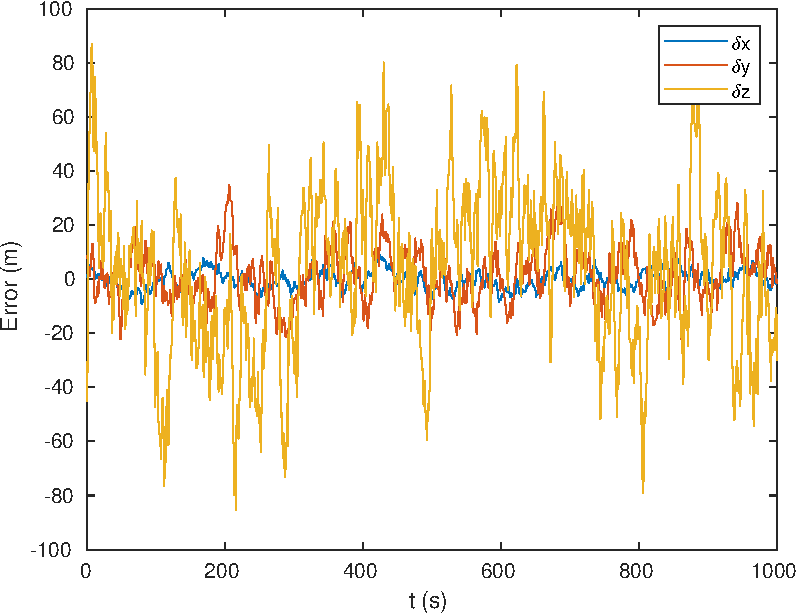
\includegraphics[width=0.5\textwidth]{navErr_ECRP.pdf}
    \caption{Position error of the navigation filter.\label{fig:err_pos}}
\end{figure}

List here the notes from your research during the week.
Your research should be aligned with the goals that you set for yourself at the start of the week.
Here's an example of a figure reference: \cref{fig:err_pos}.

    \subsection{More results}
        \lipsum[1-5]

\end{document}